\chapter{Qualitative results}

Here we include the output of our various systems on the datasets Buffy, Pascal 
and VideoPose datasets discussed in \secref{experiments}.

\section{CPS results}
\begin{itemize}
\item CPS results on Buffy \figref{buffy-cps1}
\item CPS results on Buffy \figref{buffy-cps2}
\item CPS results on Buffy \figref{buffy-cps3}
\item CPS results on Buffy \figref{buffy-cps4}

\item CPS results on Pascal \figref{pascal-cps1}
\item CPS results on Pascal \figref{pascal-cps2}
\item CPS results on Pascal \figref{pascal-cps3}
\item CPS results on Pascal \figref{pascal-cps4}
\item CPS results on Pascal \figref{pascal-cps5}
\end{itemize}

\section{ESM results}

Video pose estimation is best viewed in video:  

\begin{itemize}
\item ESM on VideoPose: \\
\url{http://www.youtube.com/watch?v=vnOh8_D3RhQ}
\item \citet{deva2011} on VideoPose: \\
\url{http://www.youtube.com/watch?v=6wNksPXoAxI}
\item \citet{eichner09} on VideoPose: \\
\url{http://www.youtube.com/watch?v=xW6rwYOywTc}
\end{itemize}

\section{LLPS results}

A sampling of results of LLPS are shown in \figref{llps1}, \figref{llps2} and 
\figref{llps3}.  Shown as ``left'' and ``right'' models are the training 
examples defining the chosen local neighborhoods.  In red boxes we highlight 
failure cases.

\begin{figure}[tb]
\begin{center}
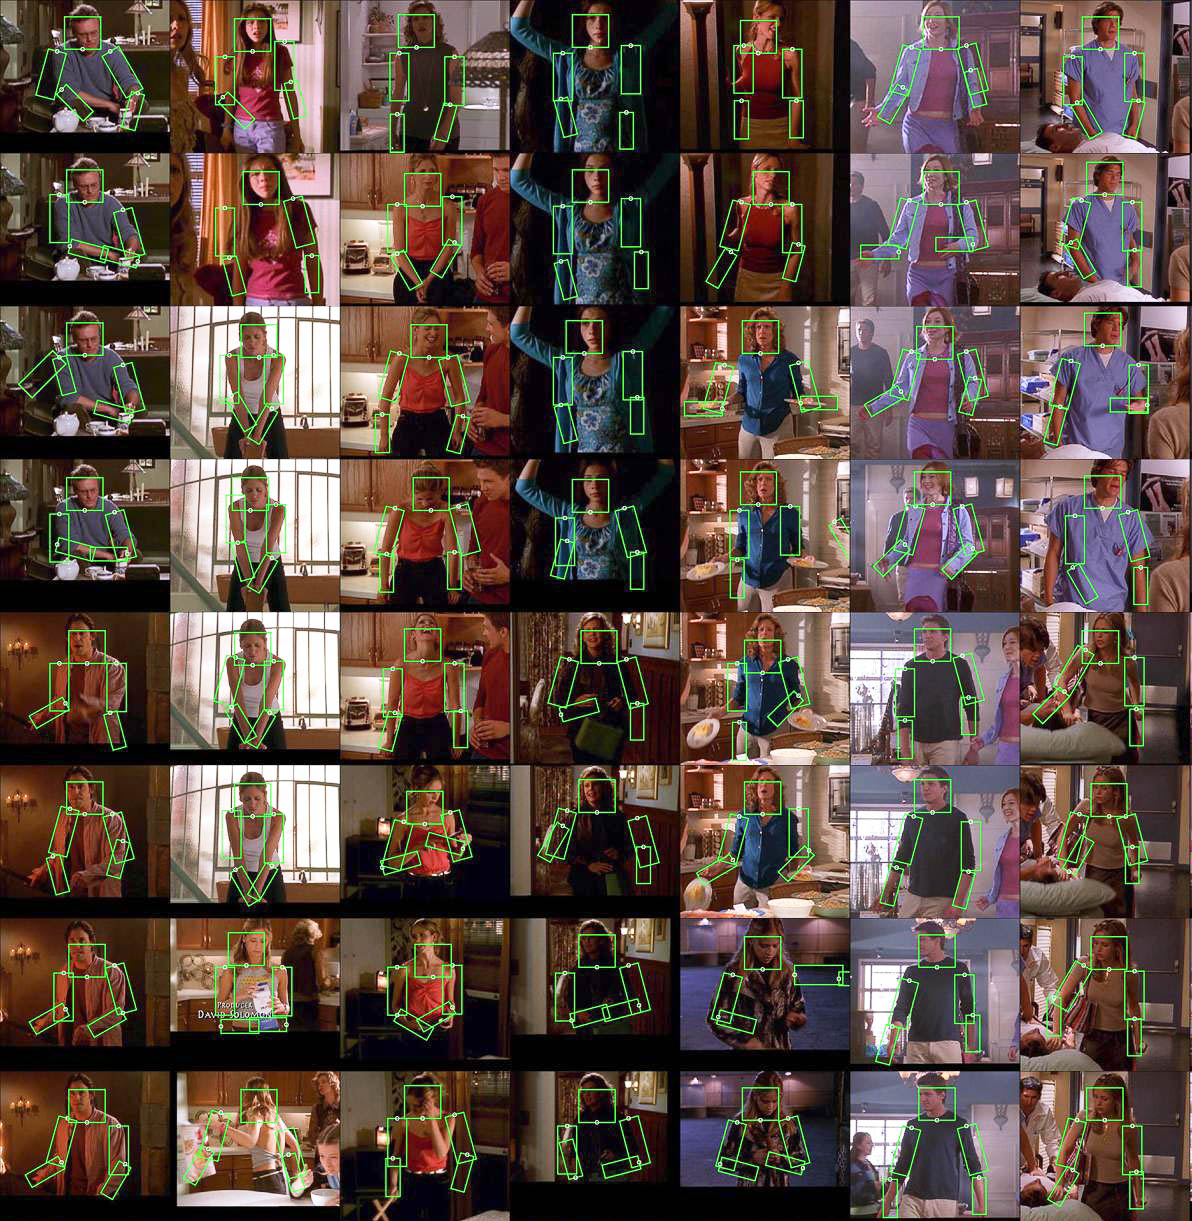
\includegraphics[width=0.99\textwidth]{figs/buffy_test_tiled_cps.jpg}
\caption[CPS results on Buffy\#1]{CPS results on Buffy \#1}
\label{fig:buffy-cps1}
\end{center}
\end{figure}

\begin{figure}[tb]
\begin{center}
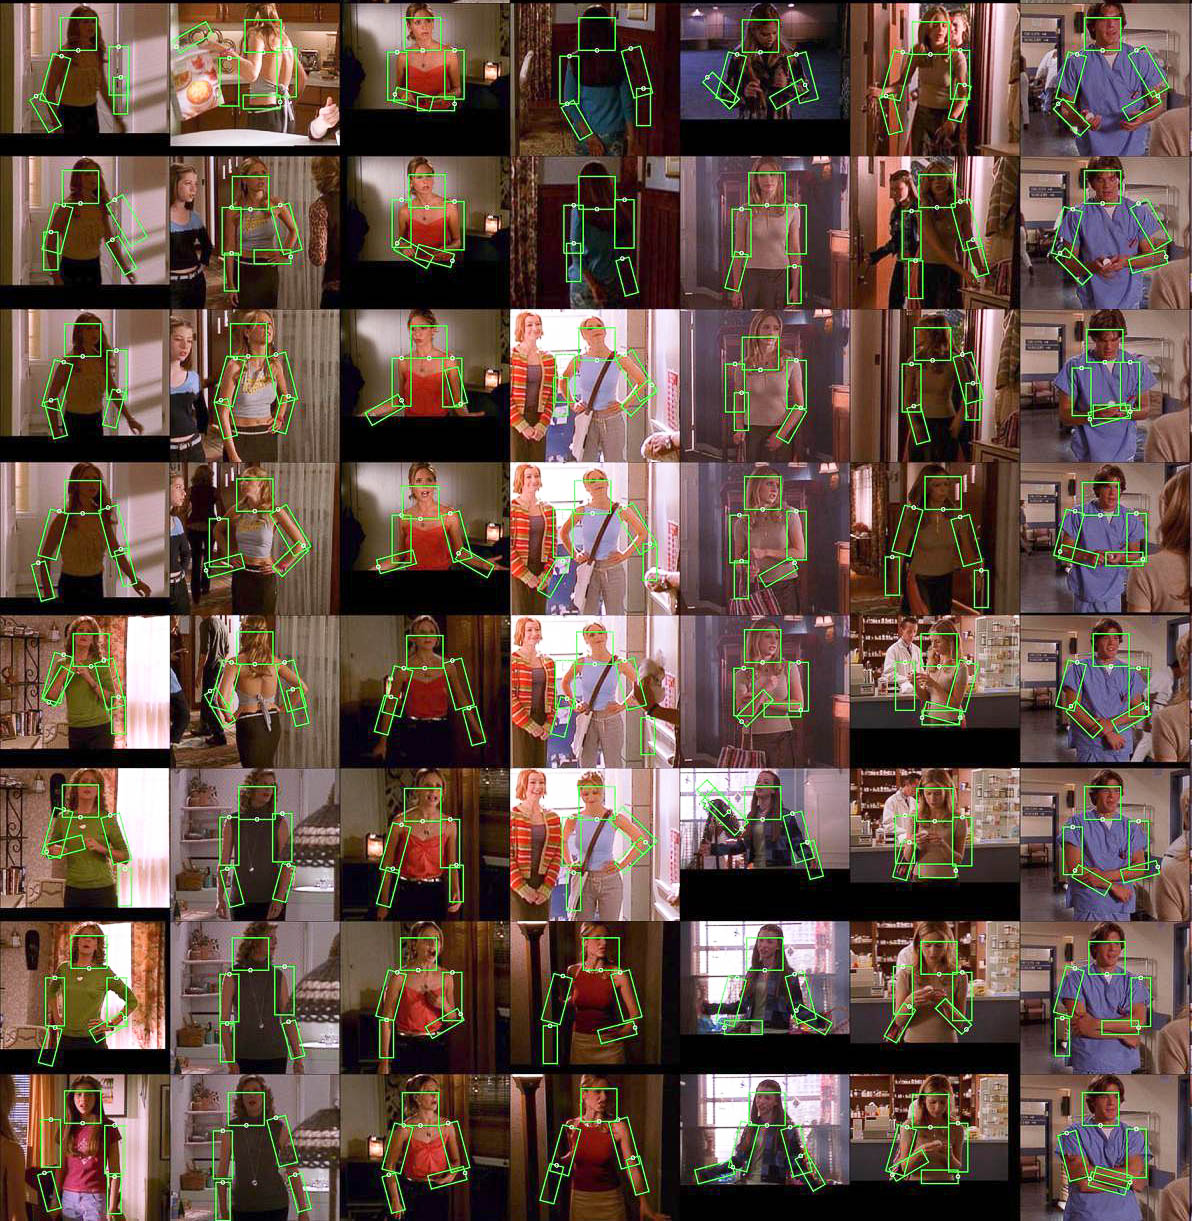
\includegraphics[width=0.99\textwidth]{figs/buffy_test_tiled_cps-2.jpg}
\caption[CPS results on Buffy\#2]{CPS results on Buffy \#2}
\label{fig:buffy-cps2}
\end{center}
\end{figure}
\begin{figure}[tb]
\begin{center}
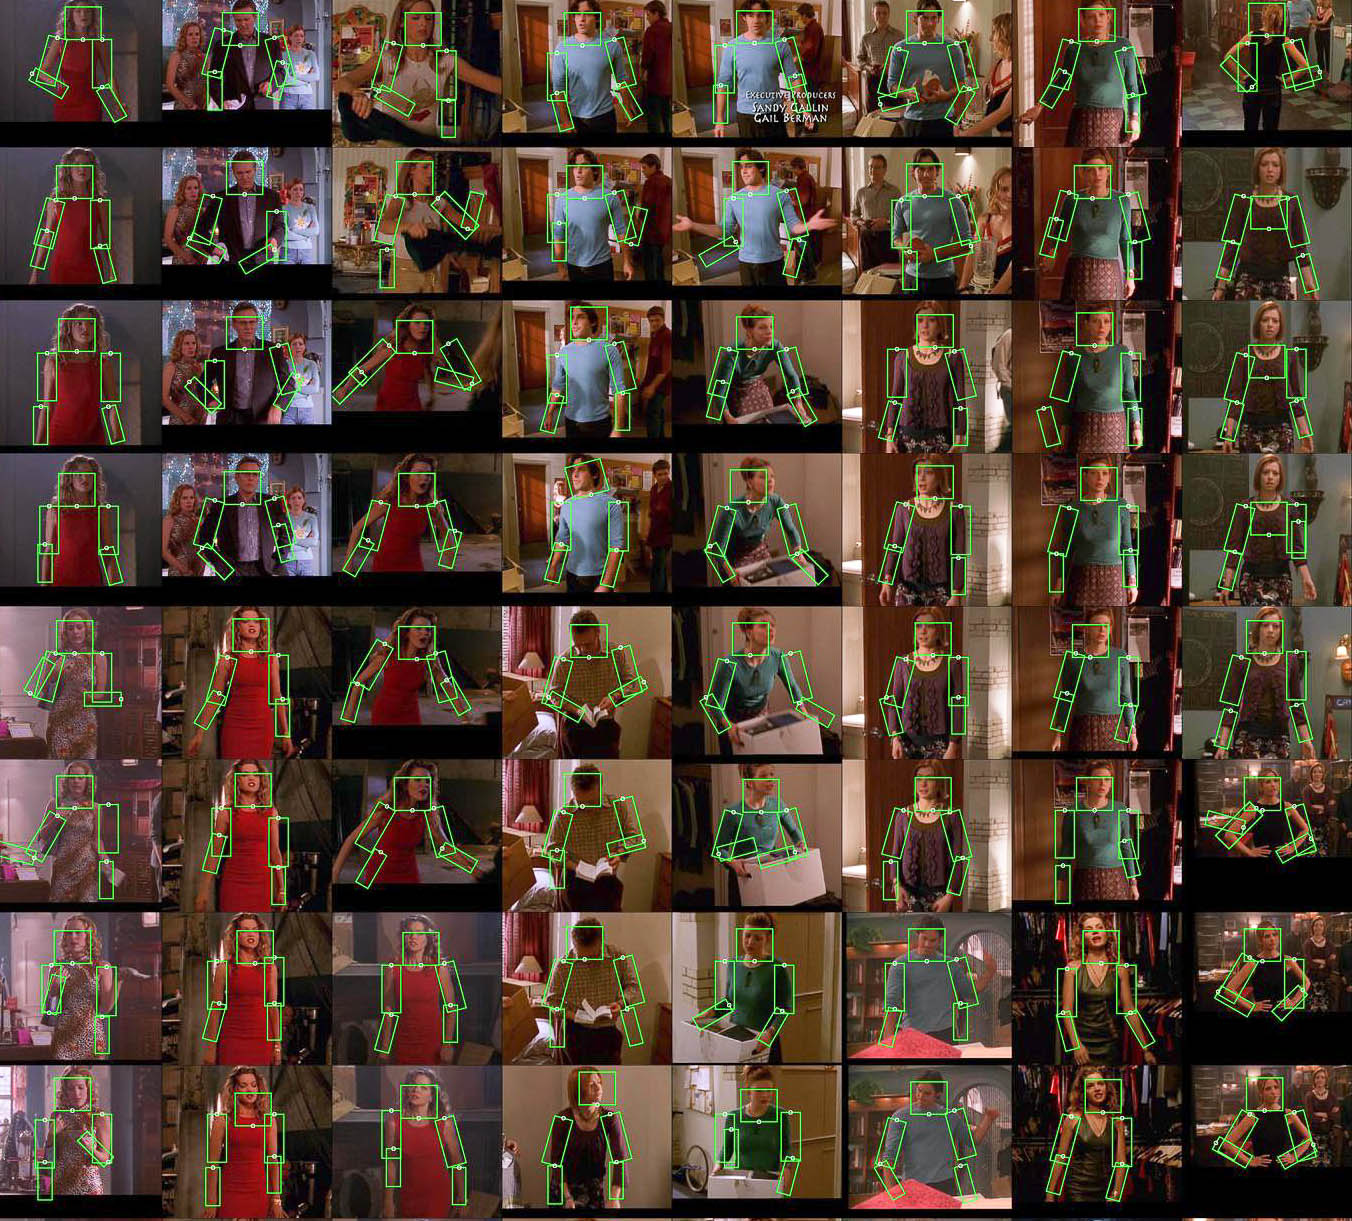
\includegraphics[width=0.99\textwidth]{figs/buffy_test_tiled_cps-4.jpg}
\caption[CPS results on Buffy\#3]{CPS results on Buffy \#3}
\label{fig:buffy-cps3}
\end{center}
\end{figure}\begin{figure}[tb]
\begin{center}
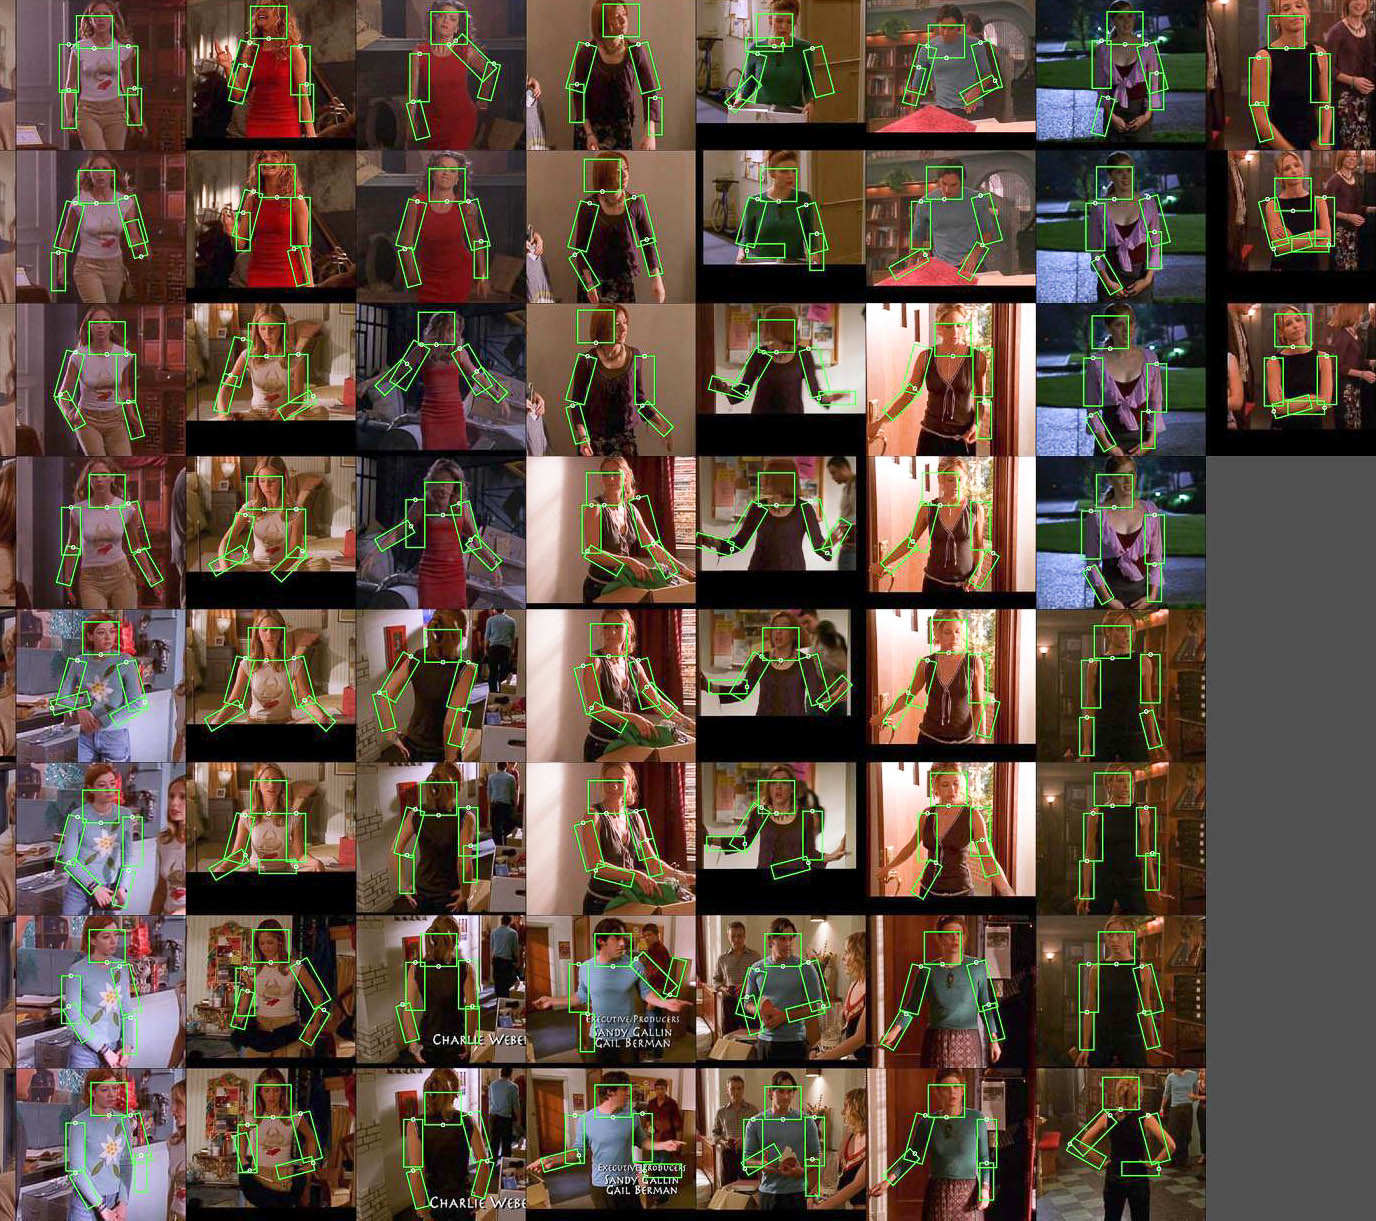
\includegraphics[width=0.99\textwidth]{figs/buffy_test_tiled_cps-3.jpg}
\caption[CPS results on Buffy\#4]{CPS results on Buffy \#4}
\label{fig:buffy-cps4}
\end{center}
\end{figure}

%%%%%%%%%%%%%%%%%%%%%%%%%%%%%%%%%%%%%%%%%%%%%%%%%%%%%%%%%%%%%%%%%%%%%%%
%%%%%%%%%                                                      %%%%%%%%
%%%%%%%%%               pascal                                 %%%%%%%%
%%%%%%%%%                                                      %%%%%%%%
%%%%%%%%%                                                      %%%%%%%%
%%%%%%%%%%%%%%%%%%%%%%%%%%%%%%%%%%%%%%%%%%%%%%%%%%%%%%%%%%%%%%%%%%%%%%%



\begin{figure}[tb]
\begin{center}
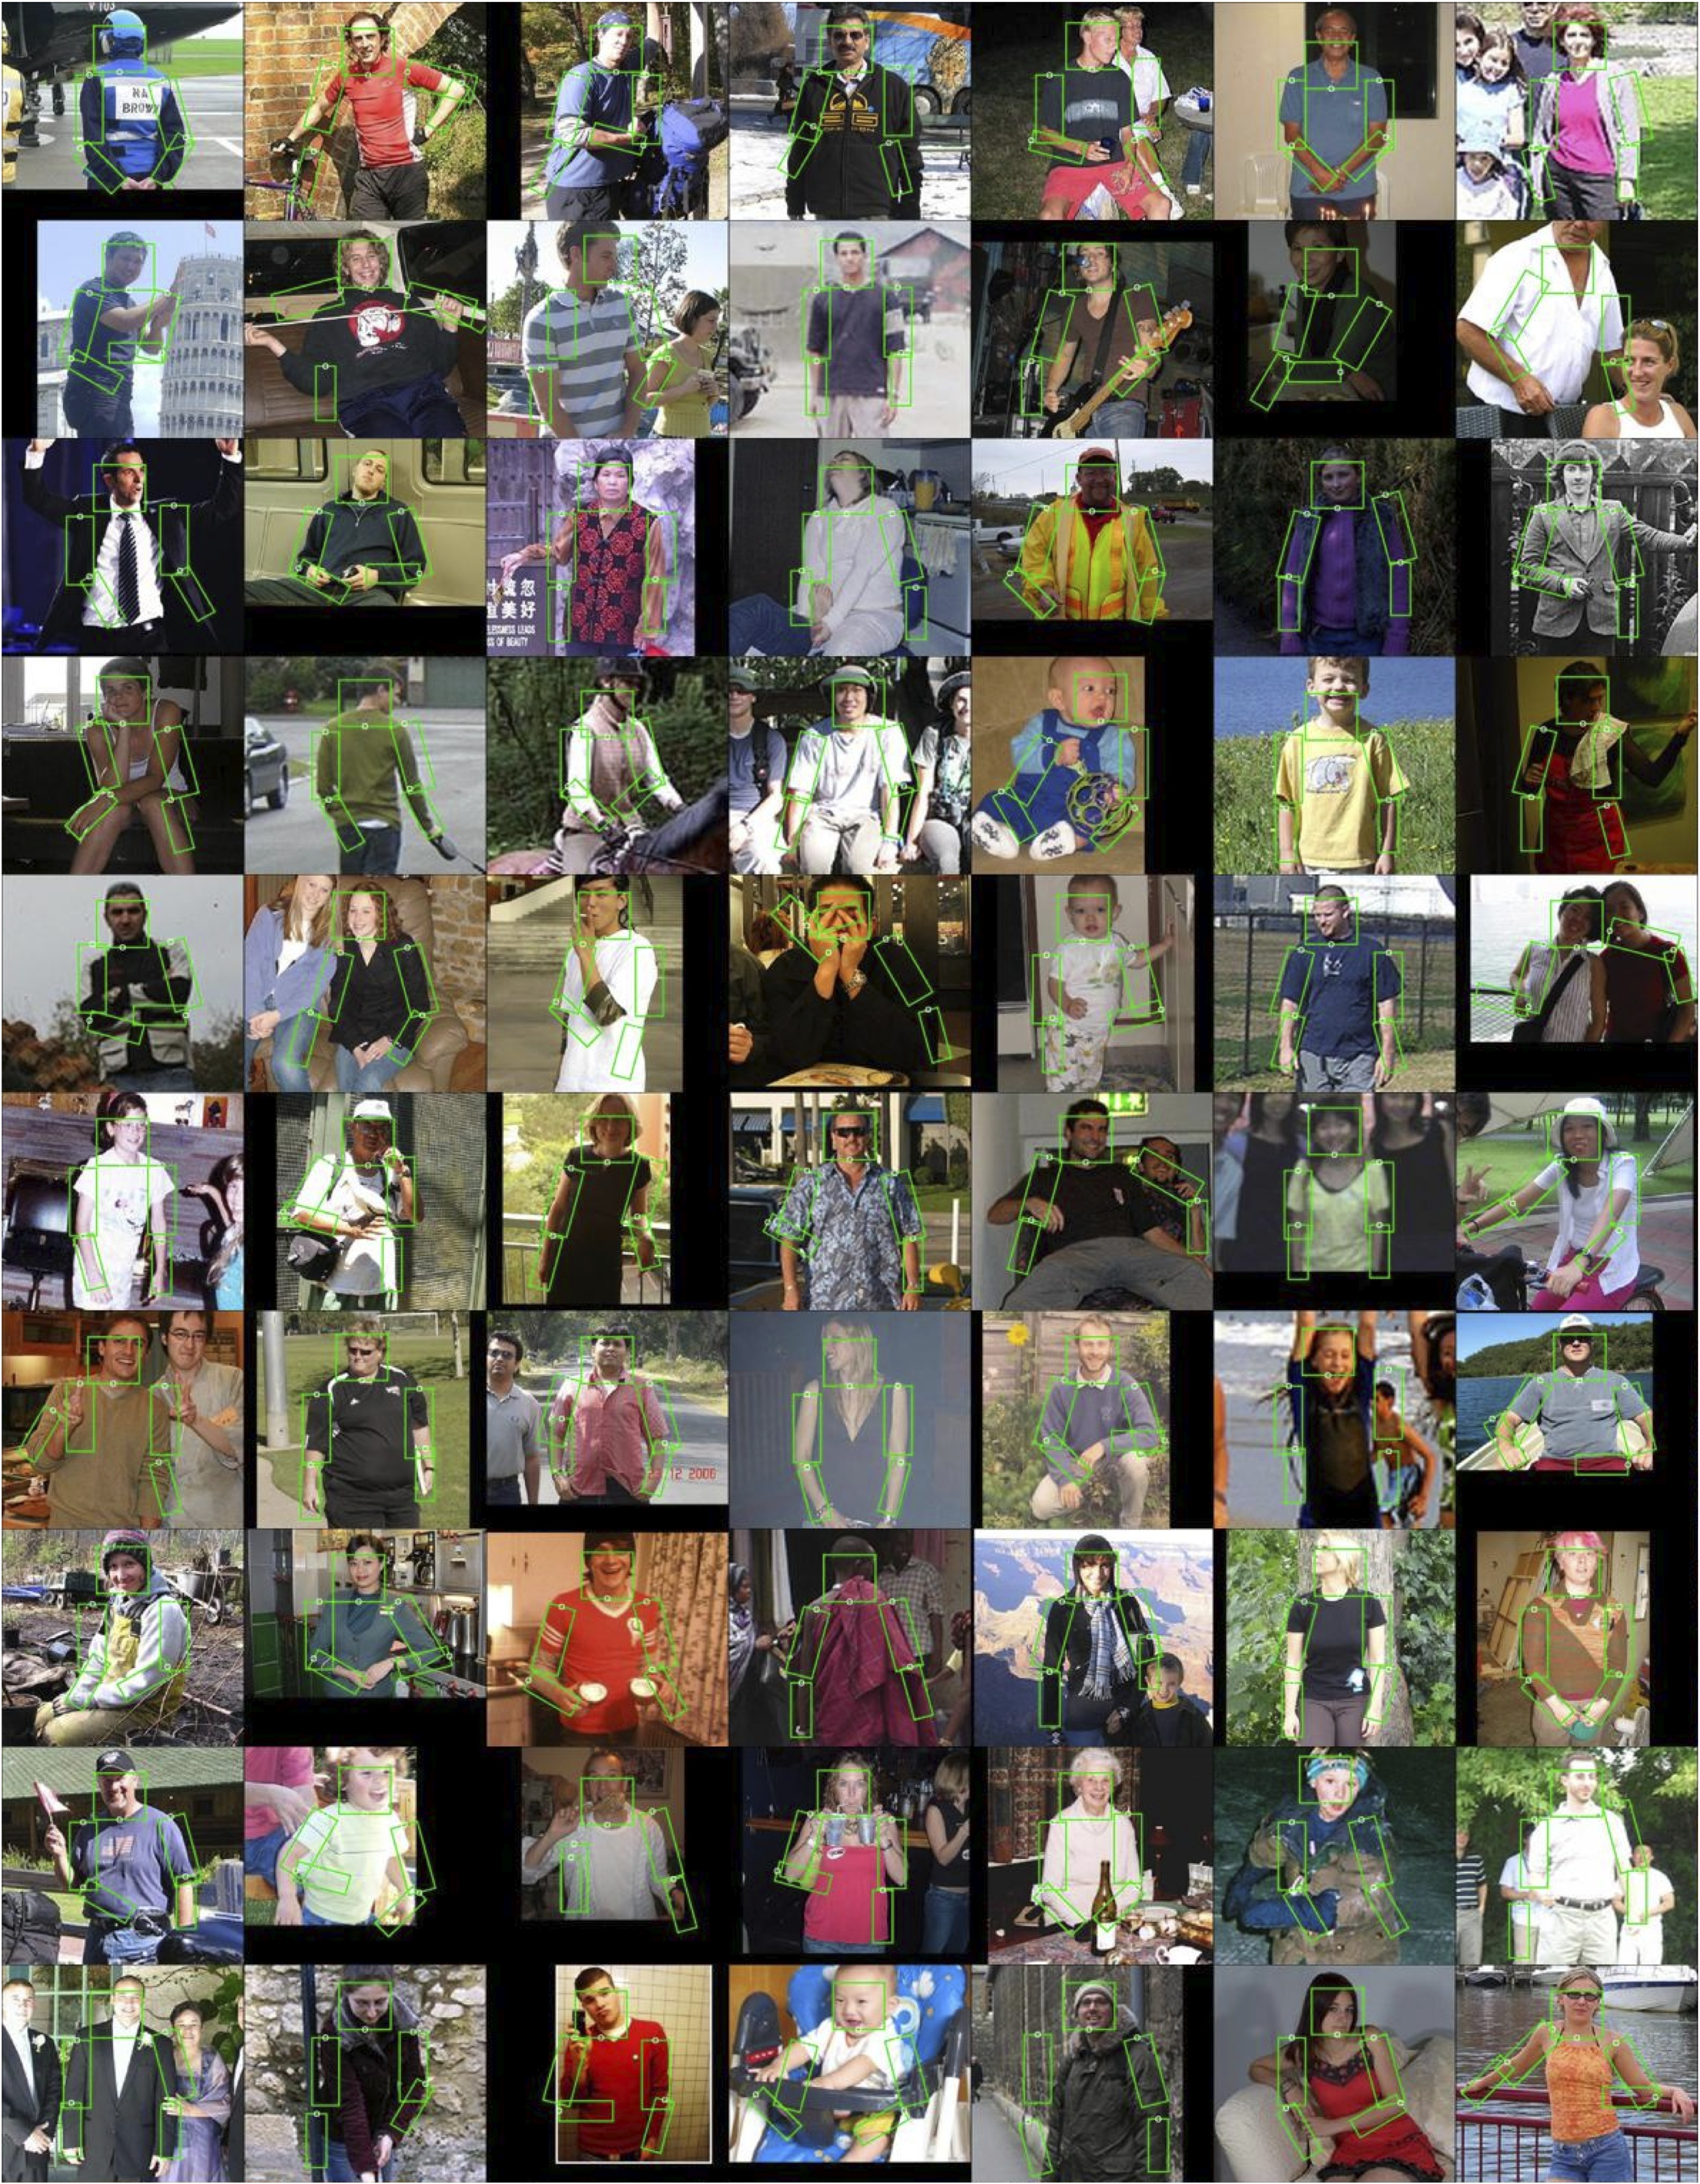
\includegraphics[width=0.99\textwidth]{figs/pascal-cps-1.jpg}
\caption[CPS results on Pascal \#1]{CPS results on Pascal \#1}
\label{fig:pascal-cps1}
\end{center}
\end{figure}

\begin{figure}[tb]
\begin{center}
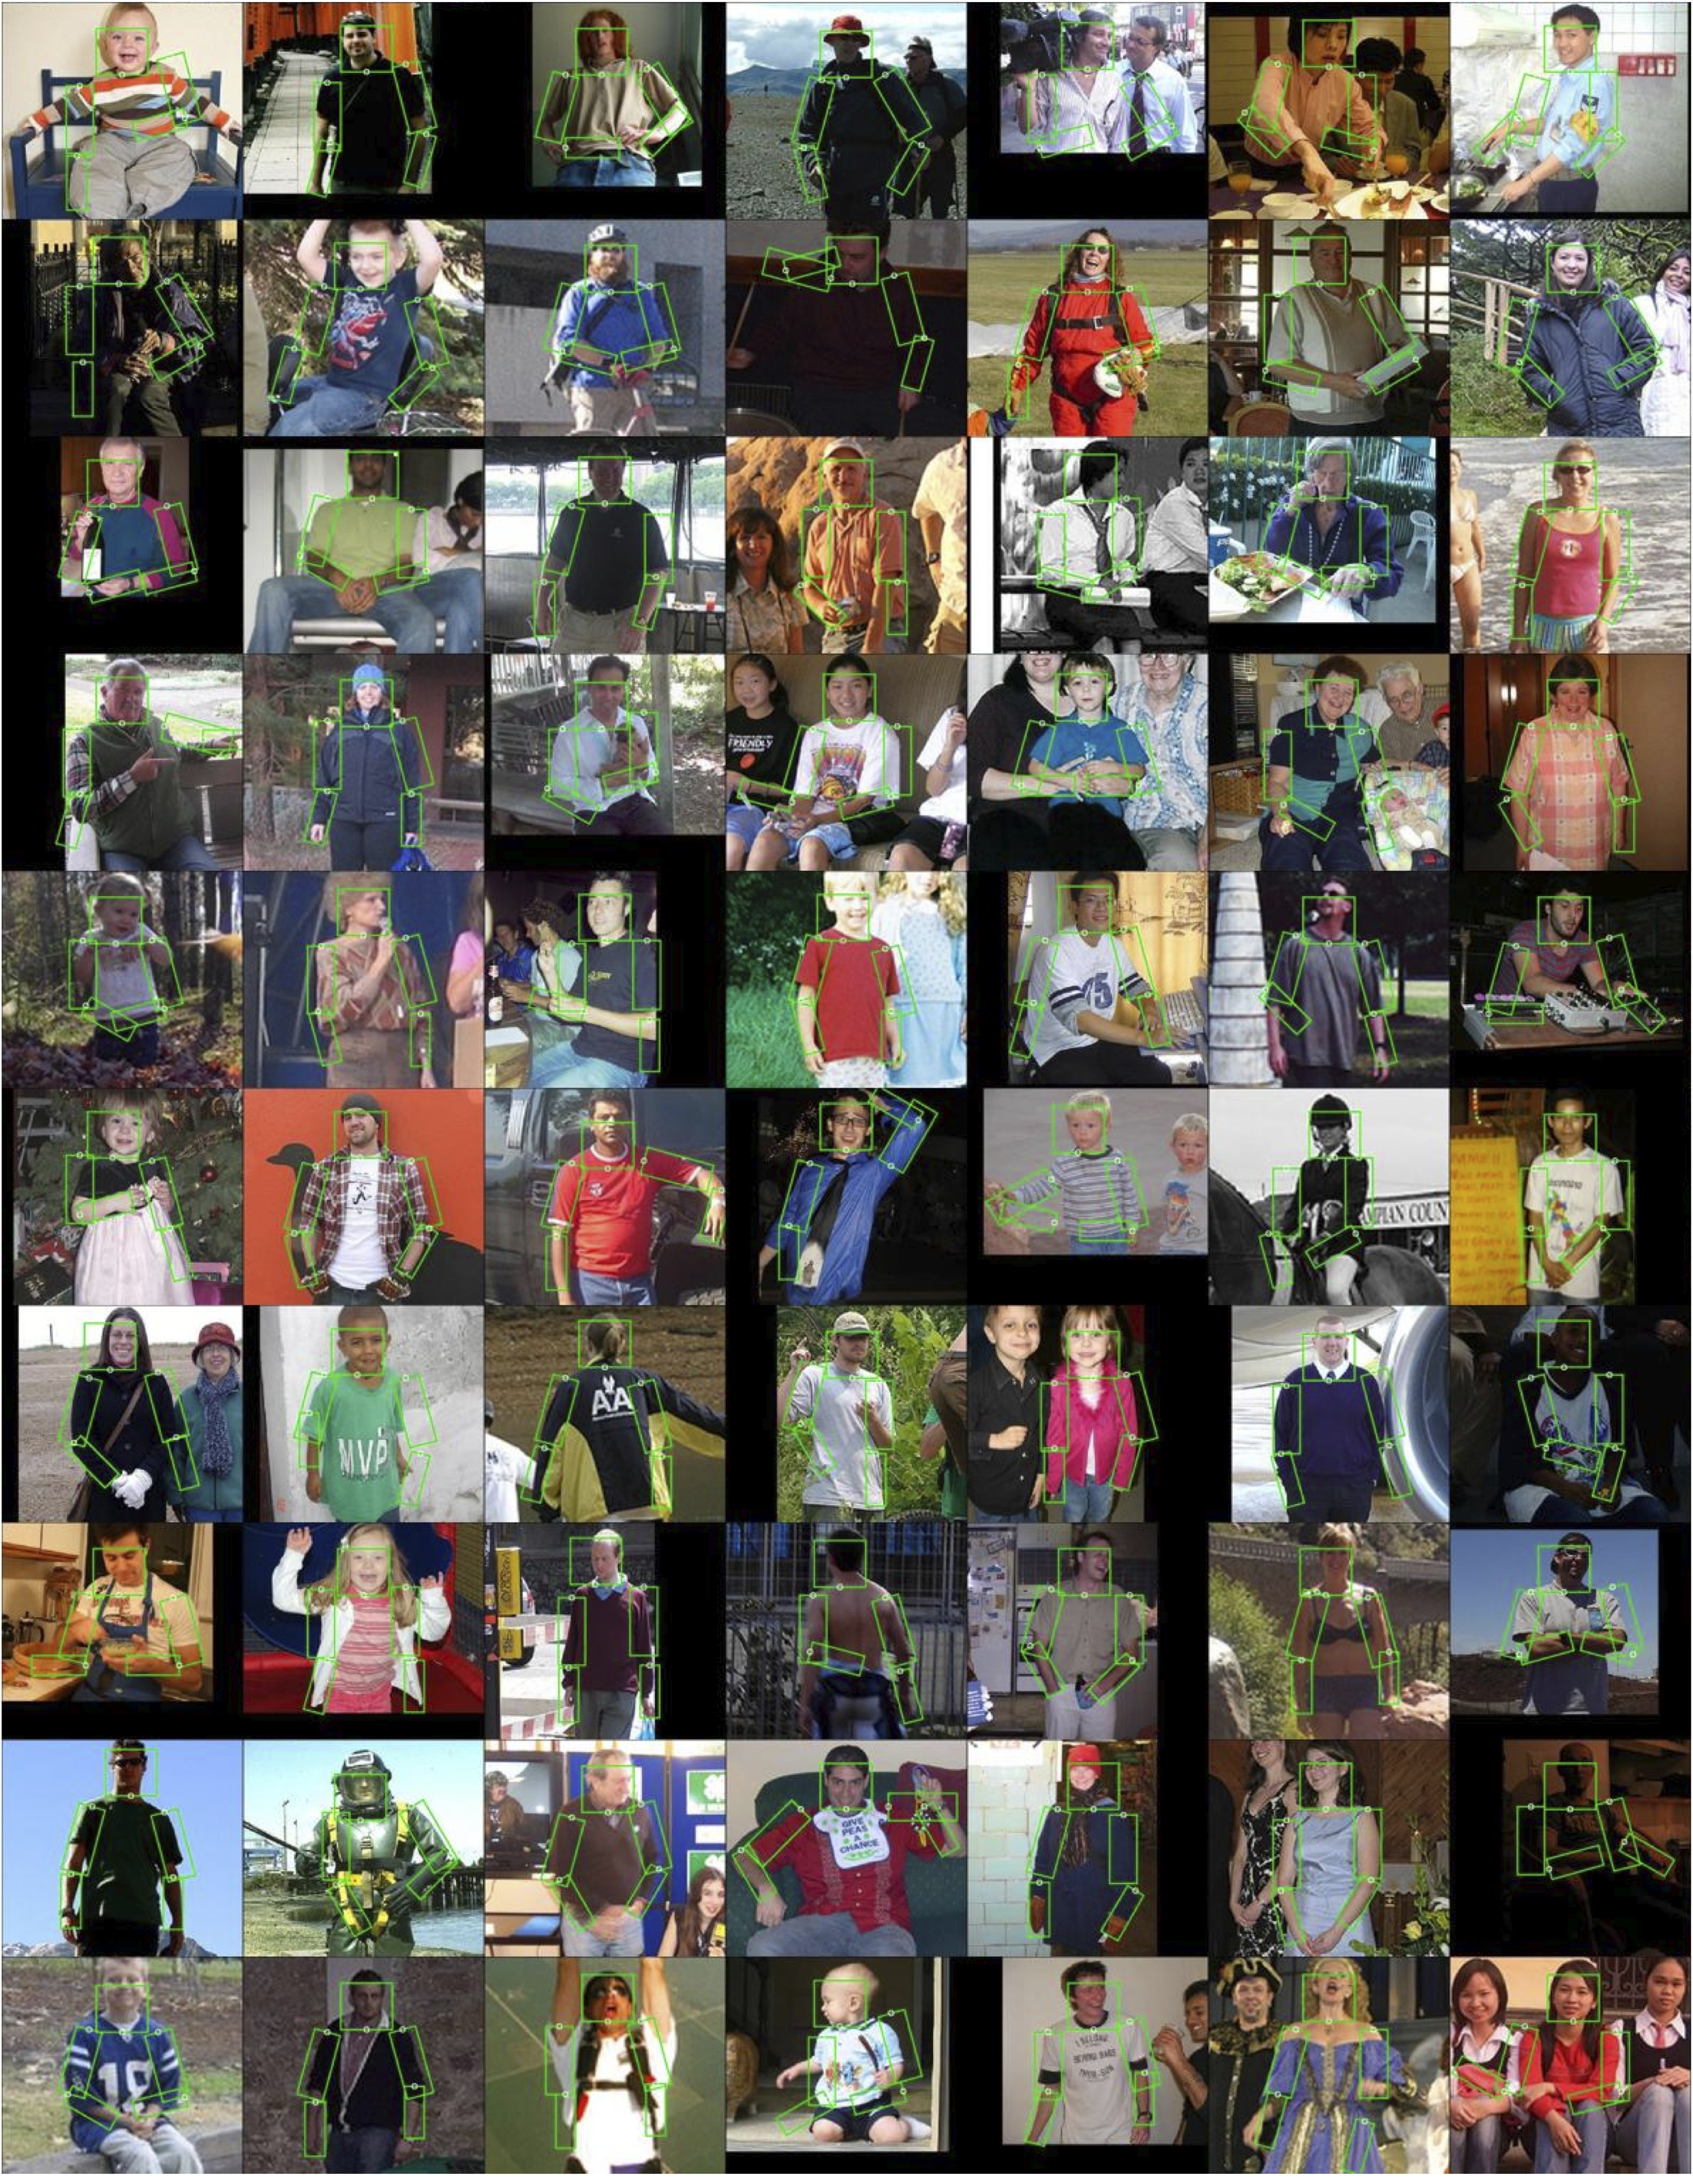
\includegraphics[width=0.99\textwidth]{figs/pascal-cps-2.jpg}
\caption[CPS results on Pascal \#2]{CPS results on Pascal \#2}
\label{fig:pascal-cps2}
\end{center}
\end{figure}

\begin{figure}[tb]
\begin{center}
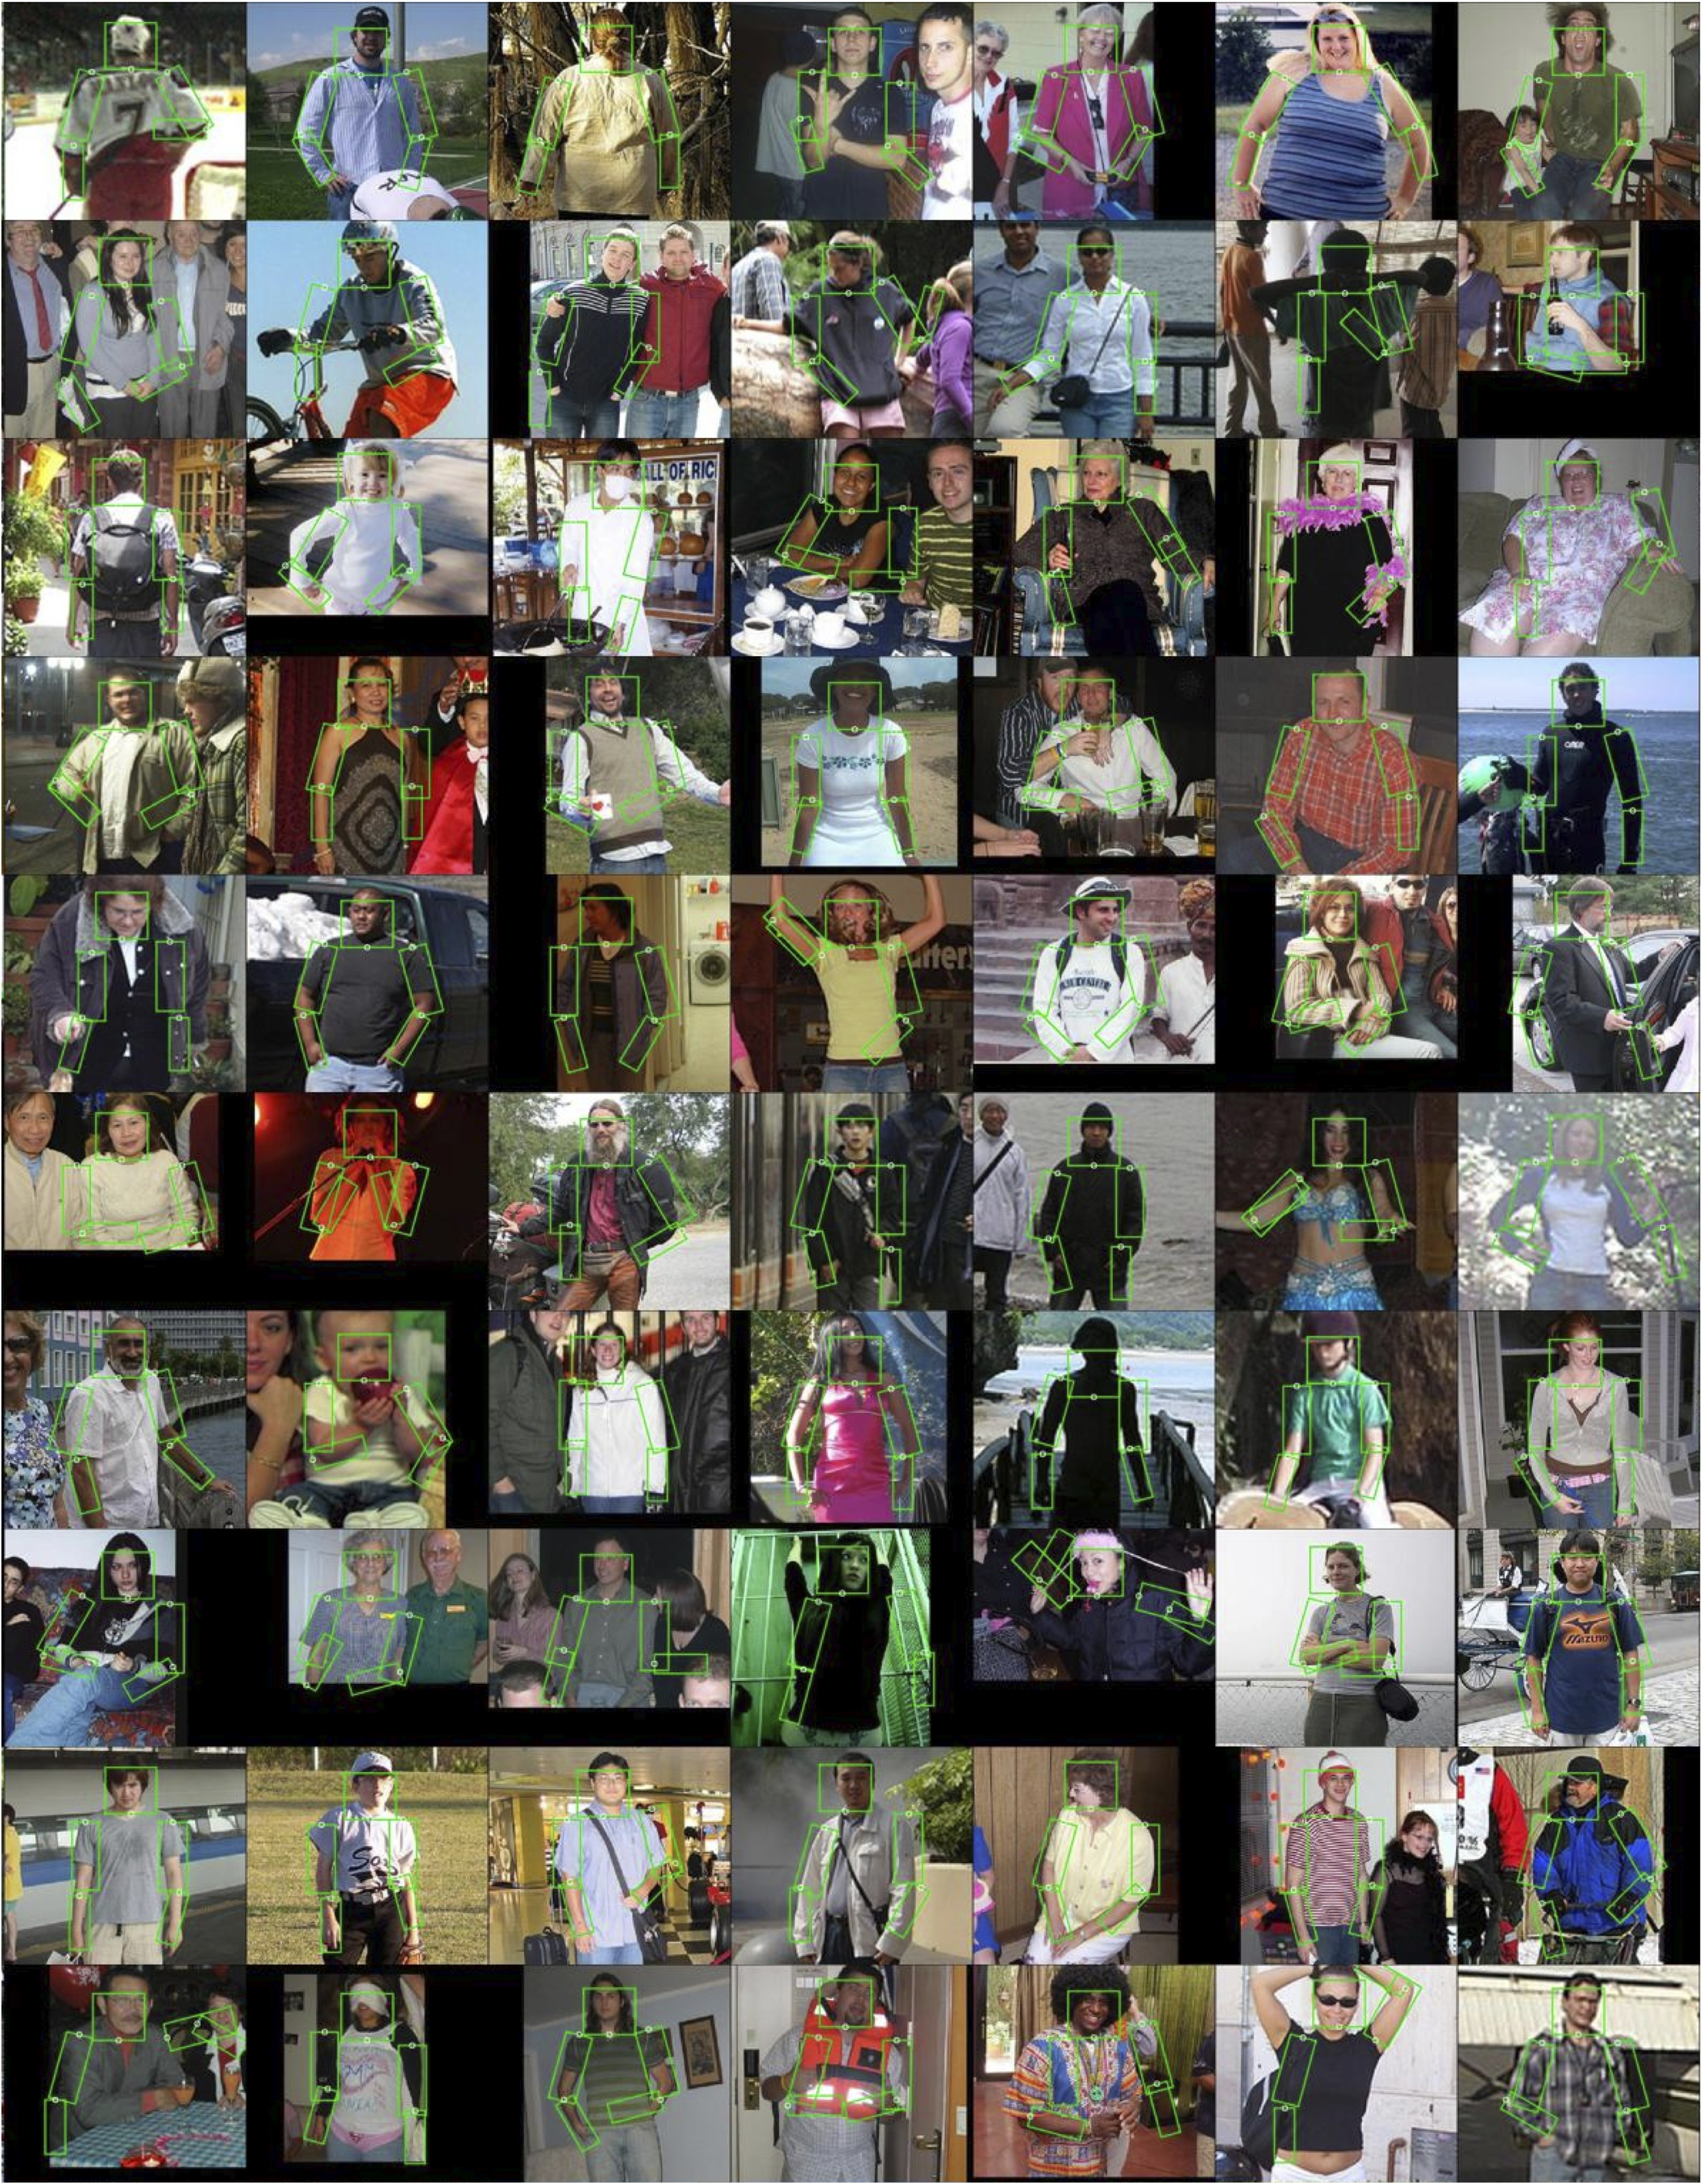
\includegraphics[width=0.99\textwidth]{figs/pascal-cps-3.jpg}
\caption[CPS results on Pascal \#3]{CPS results on Pascal \#3}
\label{fig:pascal-cps3}
\end{center}
\end{figure}

\begin{figure}[tb]
\begin{center}
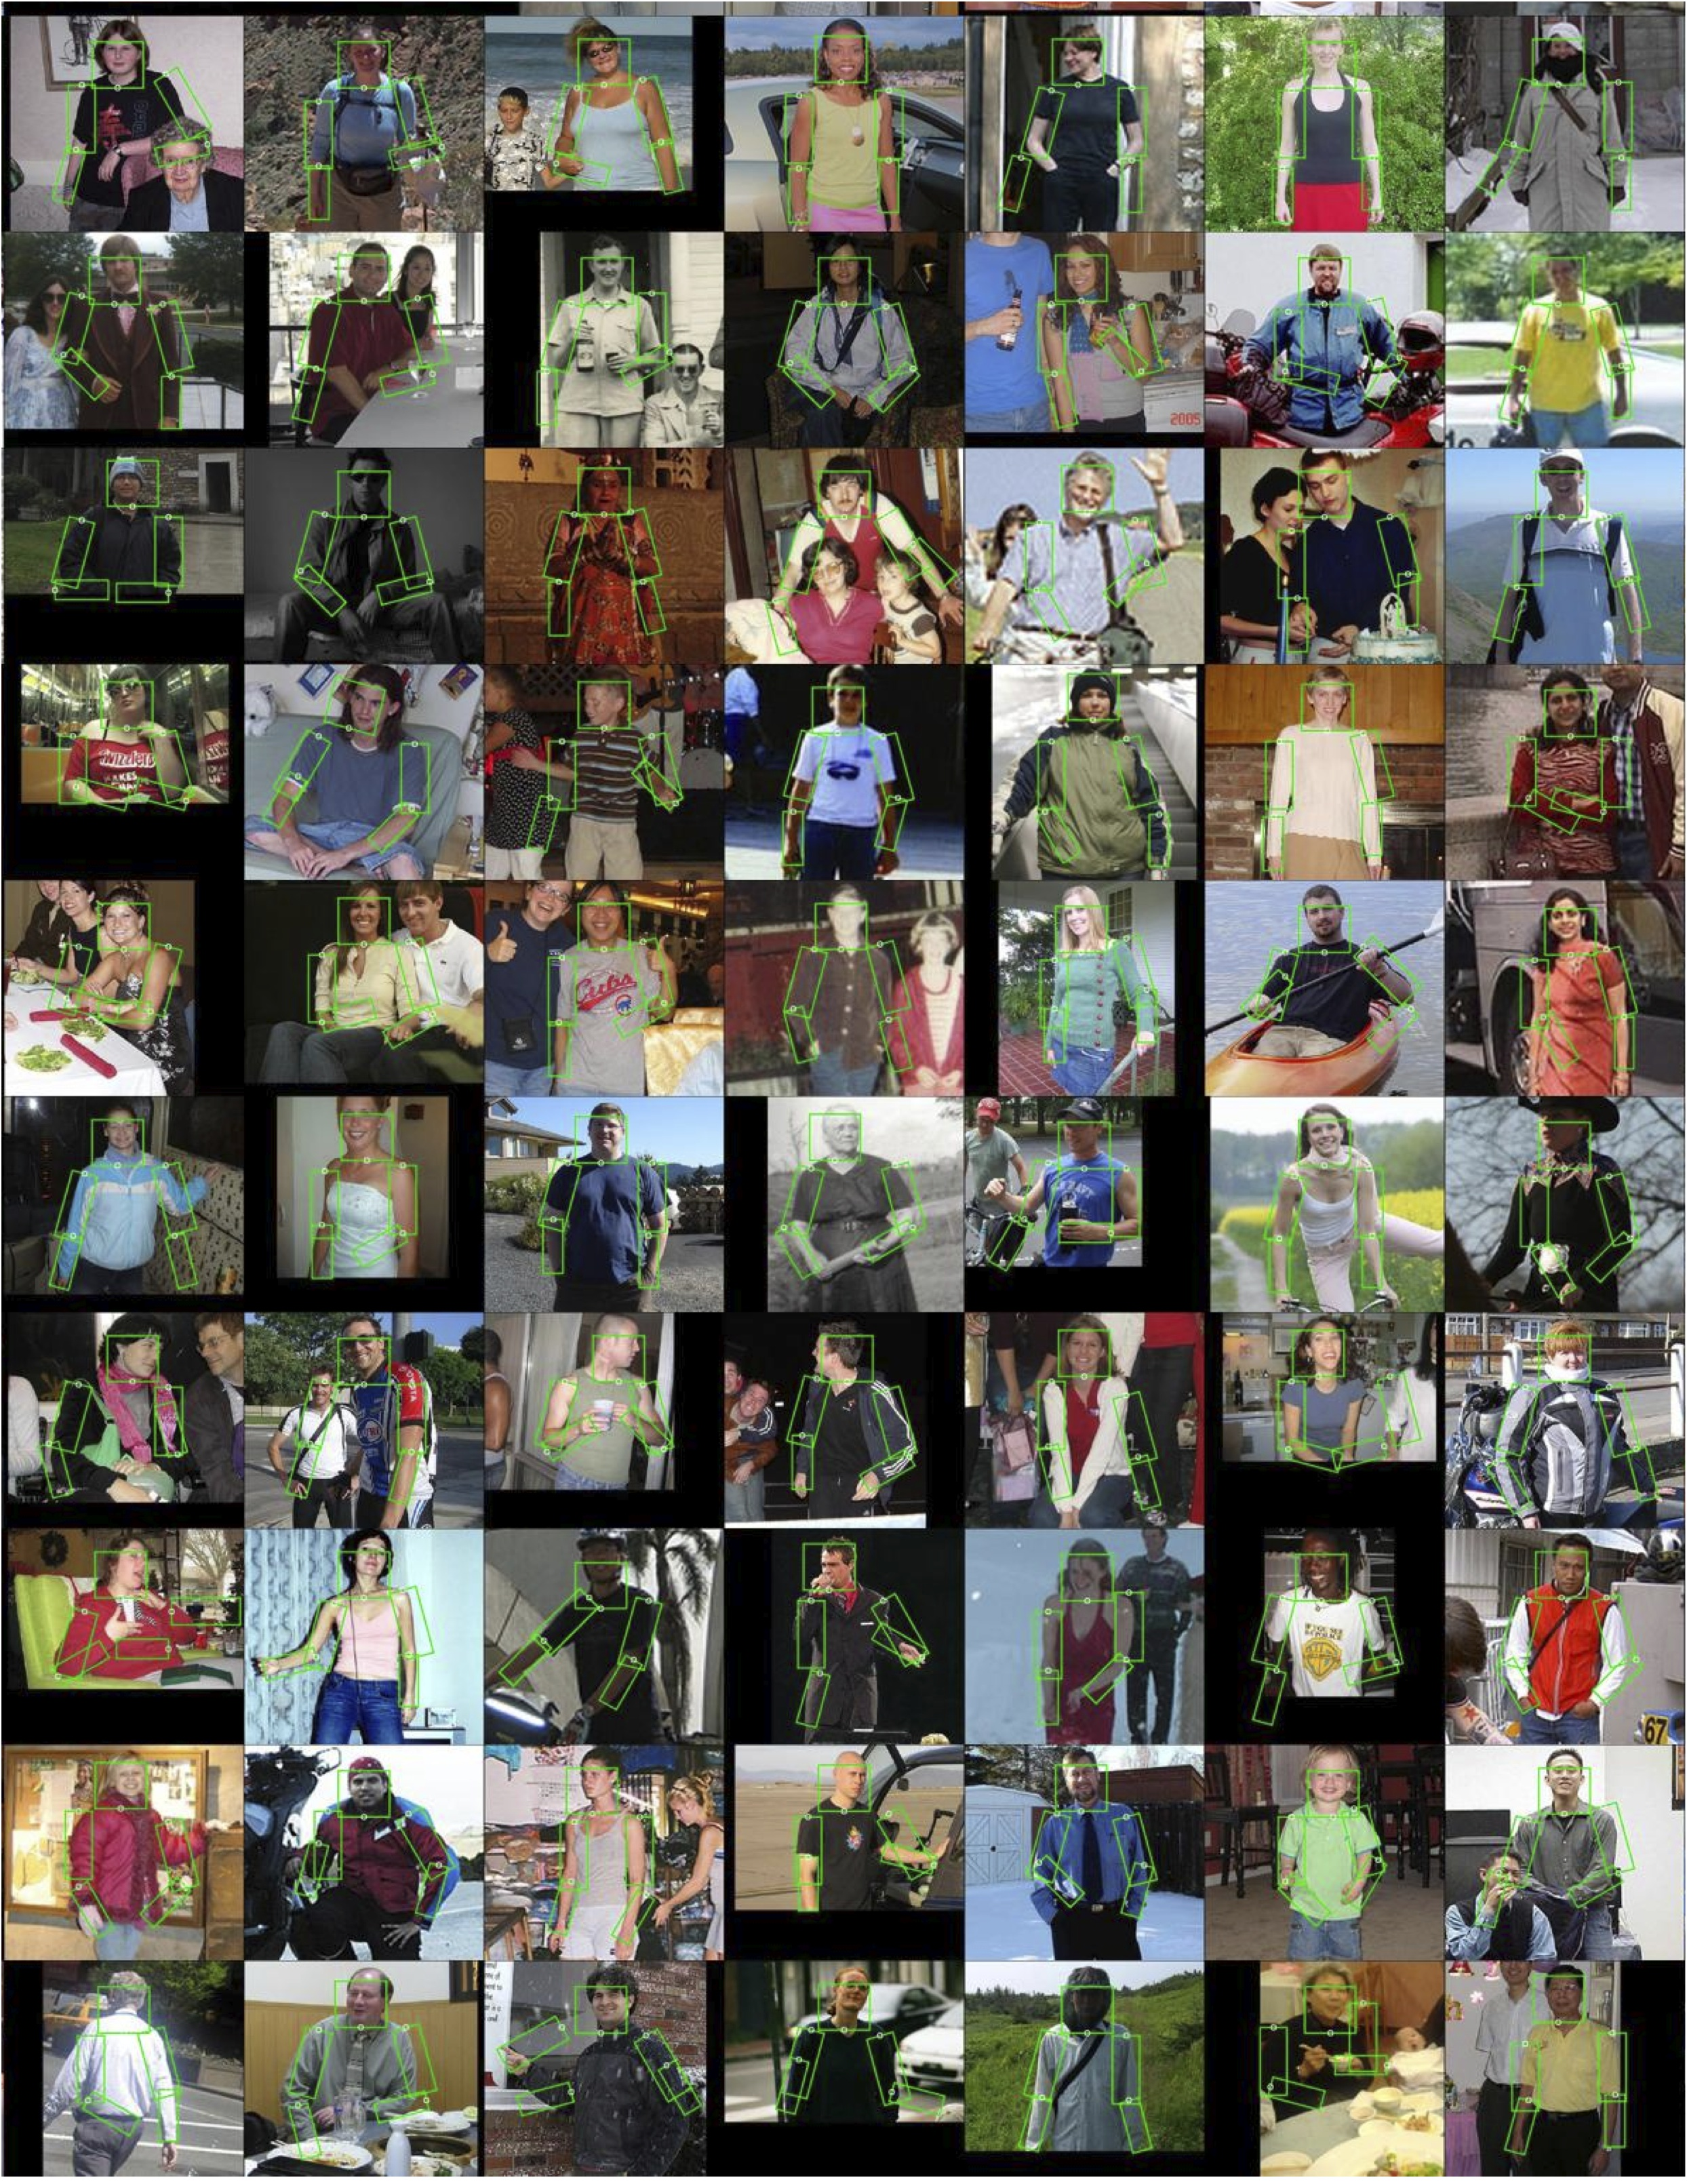
\includegraphics[width=0.99\textwidth]{figs/pascal-cps-4.jpg}
\caption[CPS results on Pascal \#4]{CPS results on Pascal \#4}
\label{fig:pascal-cps4}
\end{center}
\end{figure}

\begin{figure}[tb]
\begin{center}
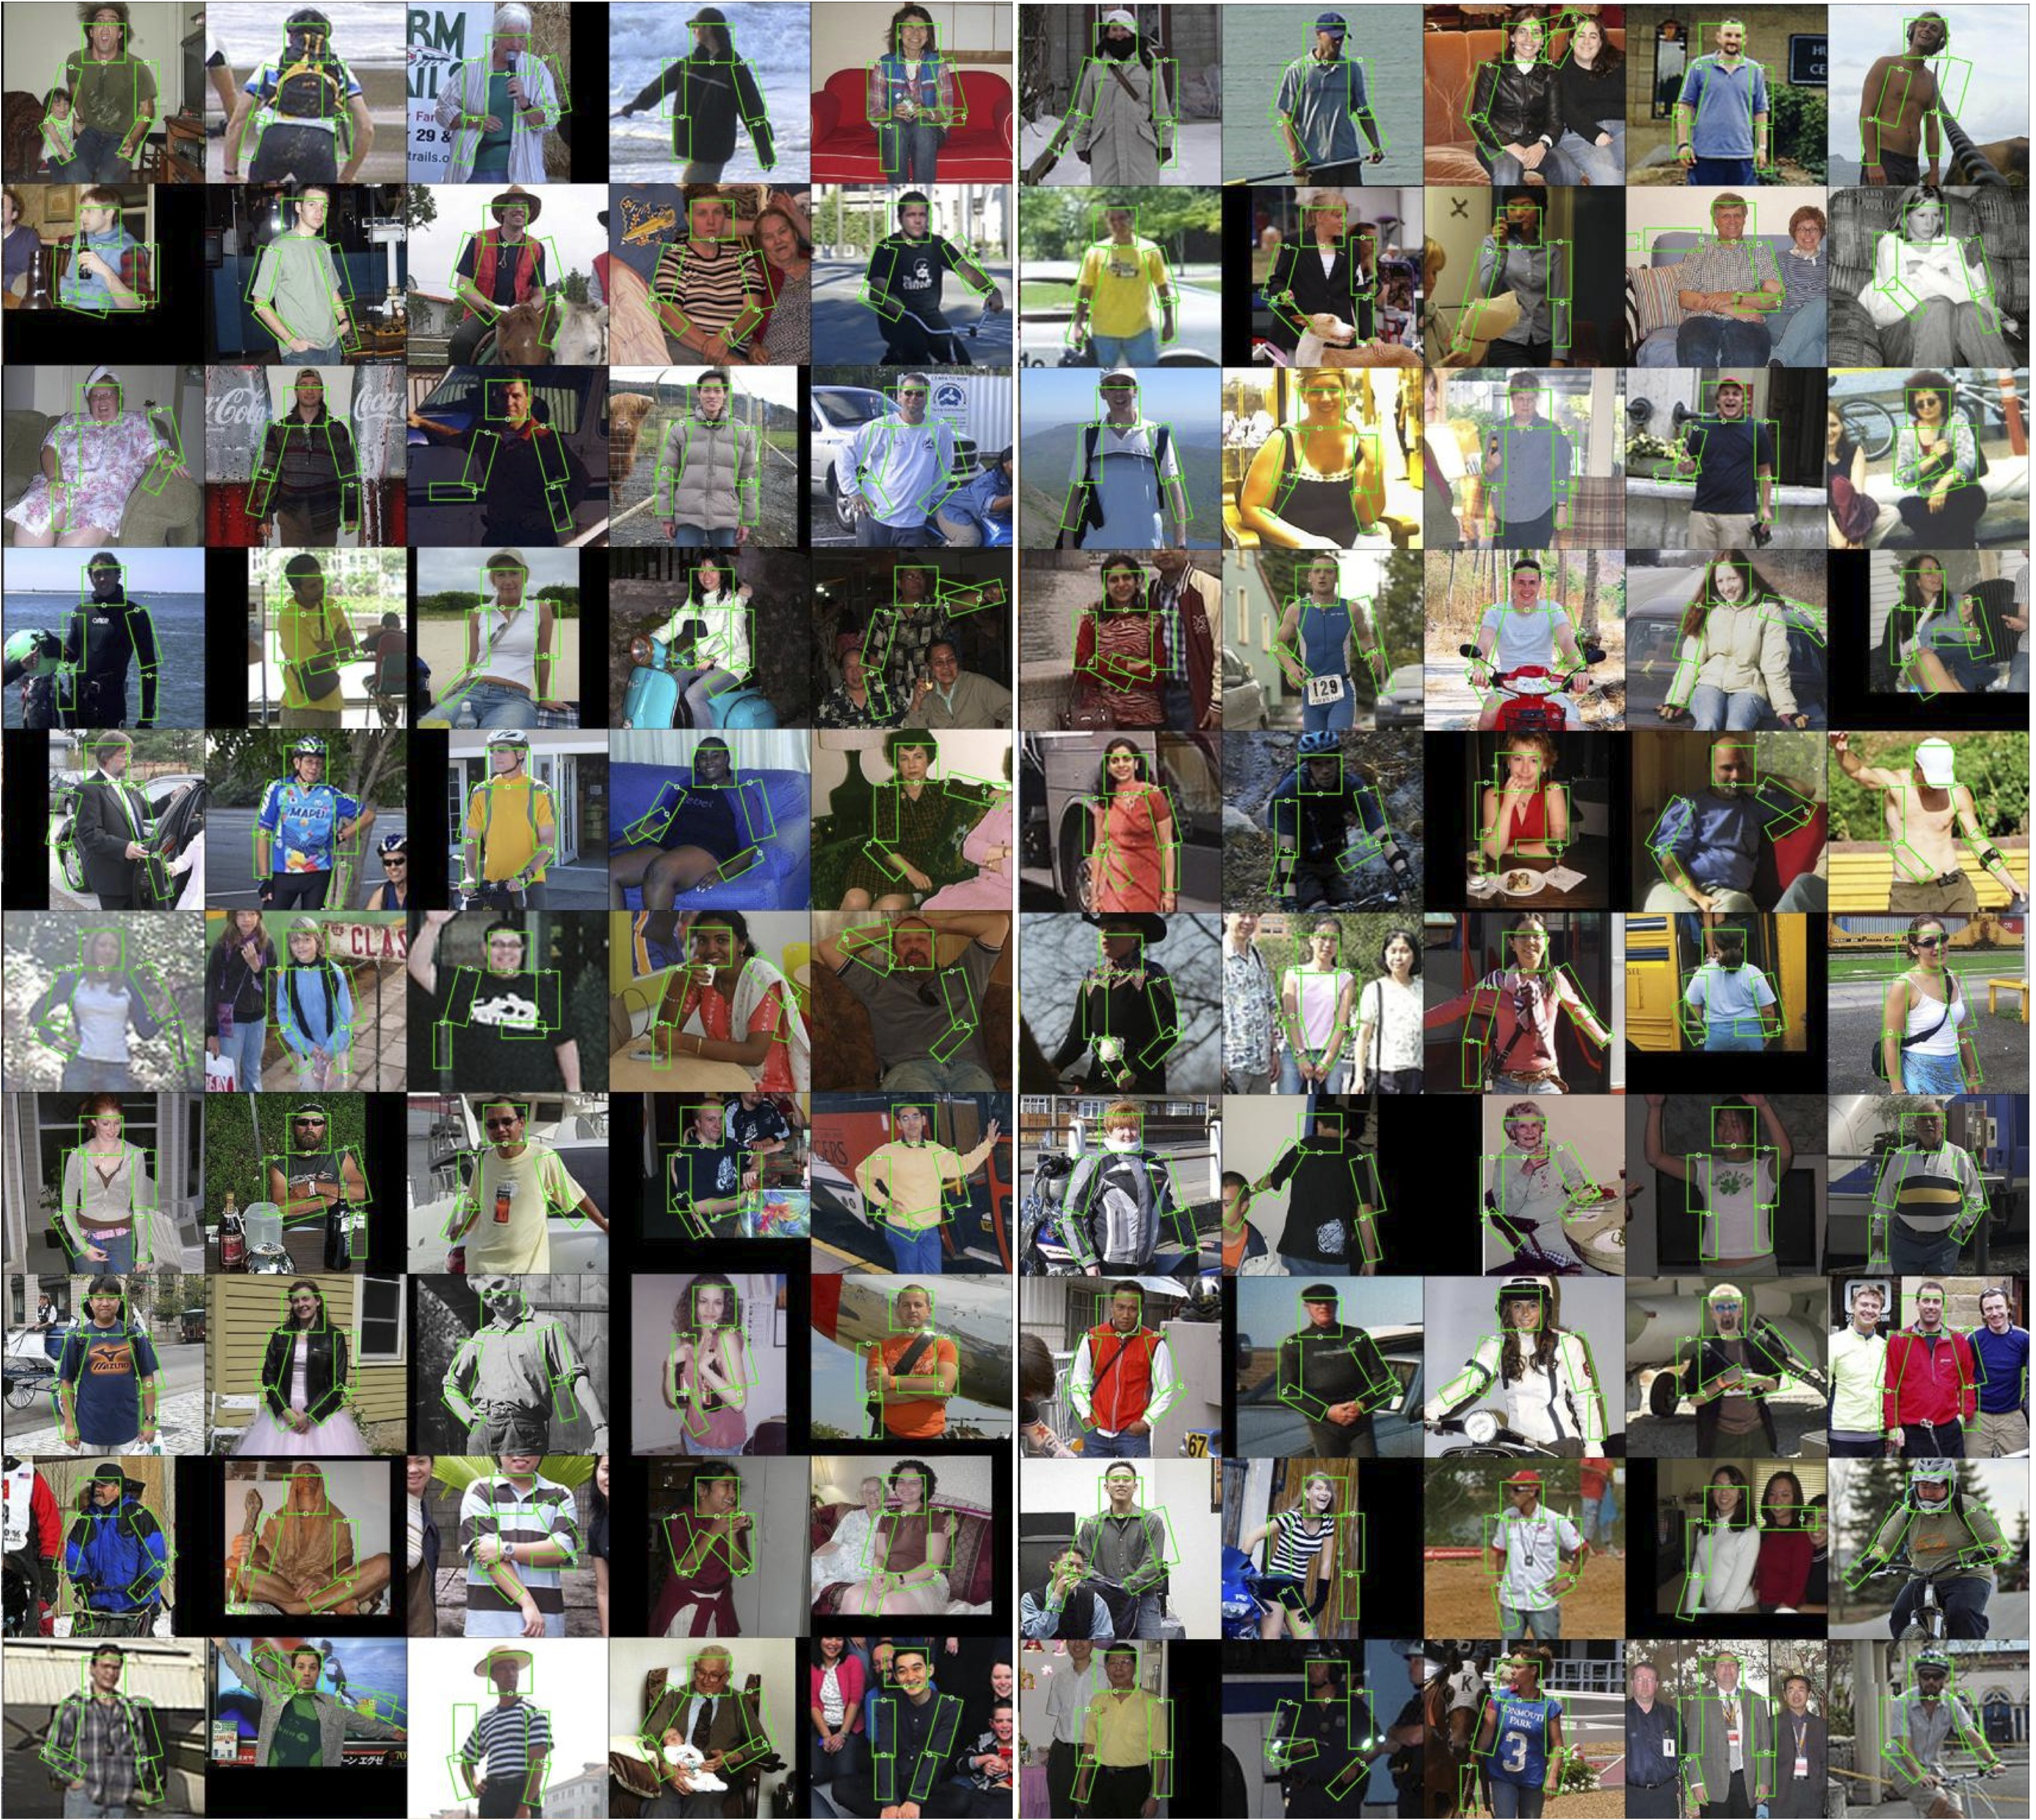
\includegraphics[width=0.99\textwidth]{figs/pascal-cps-5.jpg}
\caption[CPS results on Pascal \#5]{CPS results on Pascal \#5}
\label{fig:pascal-cps5}
\end{center}
\end{figure}

%%%%%%%%%%%%%%%%%%%%%%%%%%%%%%%%%%%%%%%%%%%%%%%%%%%%%%%%%%%%%%%%%%%%%%%
%%%%%                                                            %%%%%%
%%%%%                  LLPS                                      %%%%%%
%%%%%                                                            %%%%%%
%%%%%%%%%%%%%%%%%%%%%%%%%%%%%%%%%%%%%%%%%%%%%%%%%%%%%%%%%%%%%%%%%%%%%%%

\begin{figure}[tb]
\begin{center}
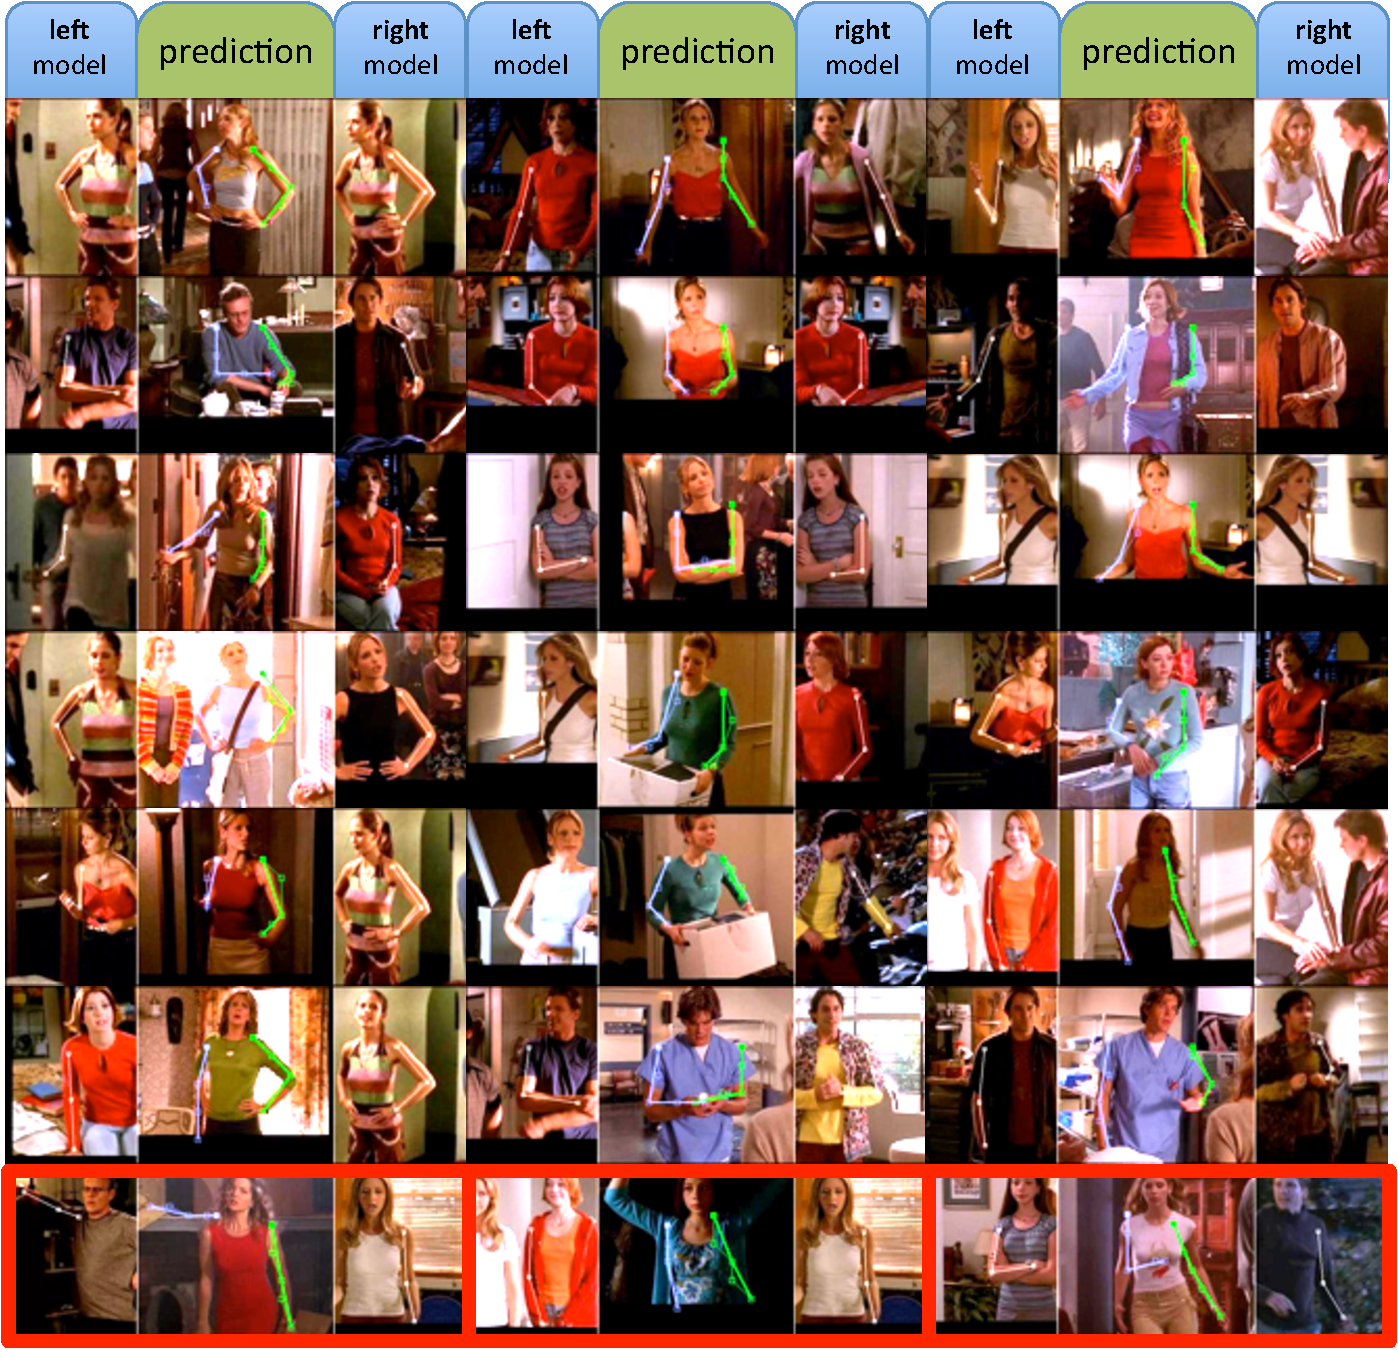
\includegraphics[width=0.99\textwidth]{figs/llps-qual-buffy.pdf}
\caption[LLPS results on Buffy]{LLPS results on Buffy}
\label{fig:llps1}
\end{center}
\end{figure}

\begin{figure}[tb]
\begin{center}
\includegraphics[width=0.99\textwidth]{figs/llps-qual-pascal.pdf}
\caption[LLPS results on Pascal]{LLPS results on Pascal}
\label{fig:llps2}
\end{center}
\end{figure}

\begin{figure}[tb]
\begin{center}
\includegraphics[width=0.99\textwidth]{figs/llps-qual.pdf}
\caption[More LLPS results.]{More LLPS results.}
\label{fig:llps3}
\end{center}
\end{figure}



